\documentclass[conference]{IEEEtran}
\usepackage[utf8]{inputenc}
\usepackage{amsmath}
\usepackage{amsfonts}
\usepackage{algorithm}  
\usepackage{algorithmic}  
\usepackage{graphicx}
\usepackage{subcaption}

\title{Team 05 EECS 467 Lab 1 Report}
\author{Jonas Hirshland, Tony Pan, Nicolas Ramirez-Icaza, Yue Wu  \\\vspace*{20pt} \normalsize  September 24, 2019}

\begin{document}

\maketitle

\begin{abstract}
A mobile robot needs to move around in a physical environment. An intelligent robot can use sensory feedback to select the approriate control laws to apply to its motors for motion. One of the main challenges of motion control is selecting which control laws to use on sensory input. In this lab, we experimented with several different control laws and compared the performance of each. We have found that neither open-loop control nor relying solely on internal odometry for feedback is an effective method. A combination of odometry deduced from internal encoder readings and the robot pose estimated based on an external lidar range sensor yielded the best outcome. 
\end{abstract}


\section{Introduction}
An intelligent robot interacts with the physical environment from sensory data and actuator motion. The robot relies on internal and external sensors to decide what control laws to use for commanding the motors. A mobile robot needs a set of control laws to govern its motion based on sensory feedback. For this project, our group implemented different types of control algorithms for driving the MBot around a 1x1 meter square. 

The MBot is about 25 centimeters by 25 centimeters in size, and has a two-wheel differential drive with encoders on each wheel motor. The MBot also has a single rotating laser range-sensor at five Hertz. It is controlled by a Raspberry Pi 3 with wireless capabilities and a BeagleBone. Both the Raspberry Pi and the BeagleBone are onboard microcomputers running on the Linux Ubuntu environment.

The communication among the Beaglebone, Raspberry Pi, and other laptops while the MBot is running is achieved through the Lightweight Communications and Marshalling (LCM). The LCM is a system for exchanging messages between different processes running on computers over a UDP socket connection. Each computer can send and receive messages on seperate channels.

In this project, we will experiment and compare the results of using open loop and closed loop control with odometry and a laser range-finder (LIDAR) with MBot. 


\section{Methodology}
For each control algorithm, we commanded the MBot to drive forward for one meter and turn counterclockwise 90 degrees. In this section, we will evaluate how well the robot can complete the square traveling motion for a few times. We used VX as our visualization tool to graph the deduced (Ded) reckoning trajectory of the MBot based on odometry as a blue line, and the robot pose as a blue triangle. The visualization program also graphed the estimated robot trajectory based on laser scans as a purple line and the current pose as a purple triangle. Each vertex where the robot turns is marked with a red square. The performance of MBot under each control law will then be compared and discussed.


\subsection{System Model}
Open loop control sets motor commands completely based on an initial input, and any feedback from sensors is not taken into account by the robot.  In this investigation, we never used true open loop because each of the three methods we used to traverse the square used PID to control the wheel velocities using a closed control loop.  However, we will refer to the 1st of the three methods we attempted as open loop because the motor commander did not consider any feedback from sensors (although the PID controller for the wheel velocities did).

In a closed loop control system, the robot not only considers previous input but also sensory feedback when computing the motor output. For the closed loop control schemes, we compare sensory data gathered (1) only based on the internal motor encoders and (2) based on that from the laser range-finder, which returns external sensory feedback.

The MBot has a left and a right motor. Each motor takes a Pulse-Width Modulation (PWM) duty cycle as the input argument. The PWM controls the voltage, and the resulting velocity of each motor. Our system calculates PWM signals based on Proportional Integral and Derivative (PID) controllers. The PID controllers calculate the appropriate commands to send to the motors based on the defined error terms. 


\subsection{Odometry Model}
Odometry is the estimation of the current robot x, y coordinates and heading, or pose, based on the sensor reading. The differential drive motors on MBot returns encoder ticks and the timestamps in $\mu$ seconds. We can compute the instantaneous wheel velocities. Let $\Delta R$ be the difference between the current and the previous encoder ticks on the left wheel motor, $\Delta L$ be the change in encoder ticks since the last encoder reading on the right motor, $\Delta t$ be the elapsed time between the current and latest encoder reading in $\mu$ seconds, $v_R$ be the current instantaneous velocity of the right wheel, $v_L$ be the current instantaneous velocity of the left wheel, $\gamma_{\rm G}$ be the Gear Ratio, and $n_{\rm e}$ be the encoder resolution. The individual instantaneous wheel velocities can then be calculated by equation \ref{eq:vr}:
\begin{equation} \label{eq:vr}
v_R = \frac{\Delta R}{\Delta t} * (\frac{2\pi R}{\gamma_{\rm G}n_{\rm e}})
\end{equation} 
for the right wheel, and by equation \ref{eq:vl}:
\begin{equation} \label{eq:vl}
v_L = \frac{\Delta L}{\Delta t} * (\frac{2\pi R}{\gamma_{\rm G}n_{\rm e}})
\end{equation}
for the left wheel. Let $\Delta s$ denote the change in position, or distance traveled by MBot in meters, R be the wheel radius in meters of MBot. 
Then the change of distance can be expressed by equation \ref{eq:ds}: 
\begin{equation} \label{eq:ds}
\Delta s = (\frac{\Delta R + \Delta L}{2}) * (\frac{2\pi R}{\gamma_{\rm G}n_{\rm e}})
\end{equation}
Let $\Delta \theta$ represent the change in the MBot heading or rotation and B be the wheel base in meters. Similarly, the change in robot heading can be calculated via equation \ref{eq:dt}: 
\begin{equation} \label{eq:dt}
\Delta \theta = (\frac{\Delta R - \Delta L}{2}) * (\frac{2\pi R}{\gamma_{\rm G}n_{\rm e}})
\end{equation}

In our program, the Beaglebone continuously publishes the current time and left and right encoder ticks. The odometry program subscribes to these messages and periodically calculates the instantaneous velocities of the left and right wheels, as well as the change in position and heading of MBot as a whole. The current heading fixed between $-\pi$ and $\pi$ is calculated by equation \ref{eq:nt}.
\begin{equation} \label{eq:nt}
\theta_{current} = \theta_{previous} + \Delta \theta
\end{equation}
The x coordinate of MBot is updated by equation \ref{eq:nx}.
\begin{equation} \label{eq:nx}
x_{current} = x_{previous} + \Delta s \cos(\theta_{current})
\end{equation}
In a similar method, the current y coordinate of MBot is calculated by equation \ref{eq:ny}.
\begin{equation} \label{eq:ny}
y_{current} = y_{previous} + \Delta s \sin(\theta_{current})
\end{equation}

At the most basic level, our program can send motor commands to the left and right wheels individually. To complete the task of driving straight and turning, we can abstract the two wheels away and leave it as forward and angular motion. The actual forward velocity $v$ can be calculated from encoder ticks and timestamps reading via equation. \ref{eq:vf}
\begin{equation} \label{eq:vf}
v = \frac{\Delta s}{\Delta t}
\end{equation}
The actual angular velocity $\omega$ is calculated from encoder ticks and timestamps by equation \ref{eq:w}.
\begin{equation} \label{eq:w}
\omega = \frac{\Delta \theta}{\Delta t}
\end{equation}
The desired wheel velocities for the left $v_{L_{sp}}$ and right $v_{R_{sp}}$ wheels can thus be calculated by equation \ref{eq:dvr} for the right wheel and equation \ref{eq:dvl} for the left wheel.
\begin{equation} \label{eq:dvr}
v_{R_{sp}} = v + \frac{B\omega}{2}
\end{equation}
\begin{equation} \label{eq:dvl}
v_{L_{sp}} = v - \frac{B\omega}{2}
\end{equation}

Our program applies the above equations to estimate MBot's current pose including x, y coordinates and the heading $\theta$ and calculate required wheel velocities given a $\omega$ and $v$

On the Vx visualization tool, the Ded Reckoning trajectory of MBot based on odometry traces is displayed. Ded Reckoning deduces the $(\Delta s_i, \Delta\theta_i)$ values from the encoder ticks. The trajectory visualizes MBot's perceived path, which may or may not match the exact outcome in the real-world test environment. Factors like the smoothness of the ground surface can cause the wheels to drift and lead to differences between robot's perceived trajectory and the actual trajectory.

\begin{table}[h]
\caption{The list of some of the MBot parameters our program used for the odometry and PID calculations}
\label{tab:params}
\begin{center}
\begin{tabular}{|c| c| c|}
\hline
Parameter &Description    	 &Value \\
\hline
    $\Delta t$ &Sample Time &0.01\\
    $\gamma_{\rm G}$ &Gear Ratio &20.4 \\
    $n_{\rm e}$    &Encoder Resolution &48 \\
    $w_{\rm d}$ &Wheel Diameter &0.0817 m\\
    $B$ &Wheel Base &0.223 m\\
    ${\rm F}_{\rm T}$ &Filter Threshold &30\\
    $\Delta {\rm F}_{\rm T}$ &Max Filter Difference &20\\
    $\lambda$    &Navigation Constant   &1.85    \\
    $R_{{\rm E}, \rm{sat}}$ &Range Saturation &0.01 \\
    $\kappa$    &Potential Field Constant   &12 \\
    $N$ &Number of Search Points &64\\
    $d_{\rm s}$ &Search Distance &0.10 m\\
    $r_0$ &World Radius &1.829 m\\
    $r_{\rm p}$ &Post Radius &0.12 m\\
    $r_{\rm g}$ &Closed Gate Radius &0.45 m\\
    $r_{{\rm g} {\rm o}}$ &Goal Offset &0.05m \\
    $e_{\rm T}$ &Integral Reset Threshold & $[3,3,0.7,5,0,0]$ \\
    $u_{\rm T}$ &PID Saturation & $[1,1,10,0.35,1.4,2]$ \\
    $\theta_{\rm T}$ &Turn Stop Threshold &0.01 rad\\
    $d_{\rm T}$ &Drive Stop Threshold &0.05 m\\
    $v_{\rm max,square}$ &Max Speed (Square) & 0.5 m/s\\
    $v_{\rm max,drag}$ &Max Speed (Drag Race) & 1.48 m/s\\
    $v_{\rm max,man}$ &Max Speed (Manual) & 0.6 m/s\\
    $v_{\rm max,auto}$ &Max Speed (Auto Race) & 0.5 m/s\\
    $T_{\rm square}$ &Delay (Square) & 0 s\\
    $T_{\rm drag}$ &Delay (Drag Race) & 1.3 s\\
    $T_{\rm man}$ &Delay (Manual) & 0.20 s\\
    $T_{\rm auto}$ &Delay (Auto Race) & 0.30\\
\hline
\end{tabular}
\end{center}
\end{table}


\subsection{PID Control}
A mobile robot needs to interact with the physical world with its motors based on feedback from its own sensors. We have introduced odometry as a method for MBot to sense its current pose. We then need a way for MBot to react to the sensory feedback and send motor commands. Proportional-Integral-Derivative (PID) control is an adaptive controller that determines motor commands based on feedback. 

We are representing the controls of MBot in the unicycle model. A proportional controller pushes the system in the direction opposing the error term with a maginitude proportional to error. The controller pushes the motors to adjust for error with a higher gain when the error term is large, and pushes the motor softer when the error term is small. The main drawback of a proportional controller is that it cna only increase the control signal if the error term increases, so the new system reaches equilibrium at some distance from the setpoint. The phenomenon is called steady-state offset and can be avoided by introducing an integral term to the proportional controller. A Proportioal-Integral (PI) controller avoids steady-state offset, but can exhibit overshoot and oscillation. Adding a derivative term can provide frictional damping to the system to prevent overshooting. The Proportional-Derivative (PD) controller can eliminate overshoot, but is vulnerable to noise in sensor readings. The PID controller combines a PI and PD controller, and can be tuned for optimal performance for each motor.

We tuned the PID values (proportional gain, integral, derivative, and frequency) such that each wheel can reach the desired set-point velocies most quickly but without overshooting. After reaching the set-point, our PID controller maintains the wheel velocity at the set-point. The controller is able to correct itself despite external forces such as friction or changes in the ground surface.

For the tasks of driving straight for one meter and turning counterclockwise 90 degrees, we implemented the wall-follower algorithm. We first define the error term and the first and second derivatives of the error term for each control law. We want the error term to exhibit damped spring behavior, so we model it in a second order differential equation (Equation \ref{eq:wf}, where $k_1$ is the integral term, and $k_2$ is the proportional gain.
\begin{equation} \label{eq:wf}
\ddot{e} + k_1 \dot{e} + k_2 e = 0
\end{equation} 
In the unicycle model, $u$ represents the control input to the system, $v$ and $\omega$ are the translational or forward and angular velocities, $v_0$ is the initial desired translational velocity, $e$ is the predefined error term, and $\theta$ is the heading of MBot. $H_i(e,\theta)$ observes the error term and the heading as inputs and selects the control law as output.
We note that for small values of $\theta$, $\dot{e} = v\theta$ and $\ddot{e} = v\omega$.
After solving equation \ref{eq:wf}, the control input $u$ can be represented as euqation \ref{eq:um}.
\begin{equation} \label{eq:um}
u = \left(\begin{array}{c} v \\ \omega \end{array}\right) = \left(\begin{array}{c} v_0 \\ -k_1\theta-\frac{k_2}{v_0}e \end{array}\right) = H_i(e,\theta) 
\end{equation}

While tuning the PID controller, the system has three behaviors. When the system is underdamped, the motor velocity oscillates but with decreasing amplitude, asymptotically convering to the desired set-point. When the system is overdamped, the velocity changes slowly to the desired set-point without overshooting. Ideally, a critically damped system moves as quickly as possible to the desired set-point without overshooting. A critically damped system requires that $k_1^2 - 4k_2 = 0$, so that $k_1 = \sqrt{4k_2}$. For our PID tuning process, we have set the proportional gain $k_2$ by numerous trials and $k_1$ slightly smaller than $\sqrt{4k_2}$.

\section{Results}
We have implemented several PID controllers for MBot to drive in a square. In this section, we discuss our specific implementation for each controller, the performance and outcome of the controller, and plots or figures supporting our claim. During our experiment, the closed-loop control with laser scans has yielded the best results both on the visualization tool and in real world.


\subsection{Closed-Loop Velocity Control}
The closed-loop velocity control consists of two PID controllers for the left wheel $v_{L_{sp}}$ and the right wheel $v_{R_{sp}}$.
For the 2 closed loop control schemes, the desired wheel velocities setpoints are calculated by equation \ref{eq:dvr} for the right setpoint and equation \ref{eq:dvl} for the left setpoint.
The proportional, integral, and derivative ($K_{P}, K_{I}, K_{D}$) where found by adjusting each parameter, viewing response plots, and then itterating this process.
More specifically, the response plots had time on the x-axis, and velocity on the y-axis.  We plotted the desired setpoint which, for tuning, was always a step function.
On the same graph, we plotted the actual wheel velocity deduced from the encoder ticks and elapsed time between readings.  We took care to perform the velocity calculations
on the controller Beaglebone computer to ensure the timestamps and therefore velocities were as accurate as possible.  The tuning procedure was as follows.
First $K_{P}, K_{I}, K_{D}$ were set to 0. $K_{P}$ was increased until the the velocity overshot the setpoint and then converged to a velocity lower than the setpoint after several oscillations.
This lower velocity was the steady state error.  To eliminate the steady state error the $K_{I}$ term was increased until this error dissapeared.
At this point we had a functional controller that overshot the setpoint slightly.  The final step was to tune $K_{D}$ to minimize this overshoot.  We tried different values for
$K_{D}$ resulting in over-damped, underdamped, and critically damped convergence to the setpoint. The final PID values used for the remainder of this investigation were the critically damped values.

The results of the under damped, over damped, and critically damped behaviors are graphs in figure 1-6 below.

\begin{table}[h]
\caption{Over, under and critically damped PID values for the left and right wheels}
\label{tab:params}
\begin{center}
\begin{tabular}{|c|c|c| c| c|}
\hline
Dampling & Wheel & $K_{P}$ & $K_{I}$ & $K_{D}$ \\
\hline
    Critical & Left & 1.4 &15 &0.01\\
    Critical & Right & 1.4 &15 &0.01\\
    Under Damped & Left & 1.4 &15 &0.0\\
    Under Damped & Right & 1.4 &15 &0.0\\
    Over Damped & Left & 1.4 &15 &0.05\\
    Over Damped & Right & 1.4 &15 &0.05\\
\hline
\end{tabular}
\end{center}
\end{table}

\begin{figure}
	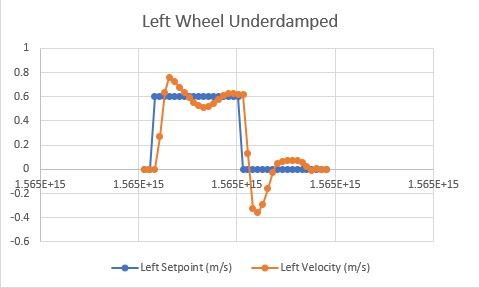
\includegraphics[width=\linewidth]{lu.jpg}
	\caption{A plot of the setpoint and velocity of the left motor exhibiting underdamped behavior}
	\label{fig:lu}
\end{figure}

\begin{figure}
	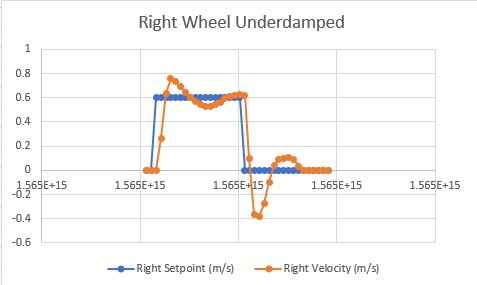
\includegraphics[width=\linewidth]{ru.jpg}
	\caption{A plot of the setpoint and velocity of the right motor exhibiting underdamped behavior}
	\label{fig:ru}
\end{figure}

\begin{figure}
	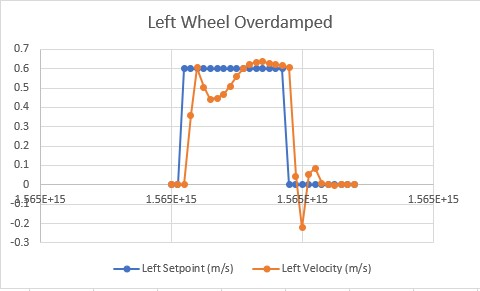
\includegraphics[width=\linewidth]{lo.jpg}
	\caption{A plot of the setpoint and velocity of the left motor exhibiting overdamped behavior}
	\label{fig:lo}
\end{figure}

\begin{figure}
	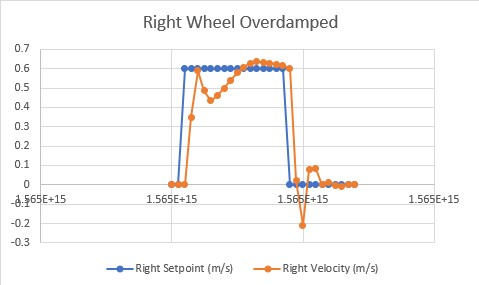
\includegraphics[width=\linewidth]{ro.jpg}
	\caption{A plot of the setpoint and velocity of the right motor exhibiting overdamped behavior}
	\label{fig:ro}
\end{figure}

\begin{figure}
	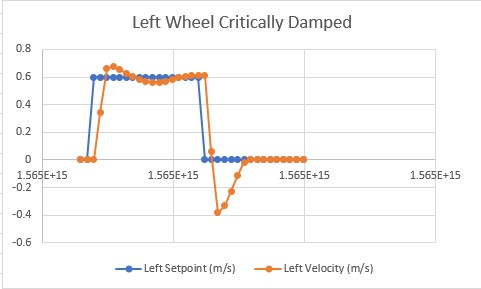
\includegraphics[width=\linewidth]{lc.jpg}
	\caption{A plot of the setpoint and velocity of the left motor exhibiting critically damped behavior}
	\label{fig:lc}
\end{figure}

\begin{figure}
	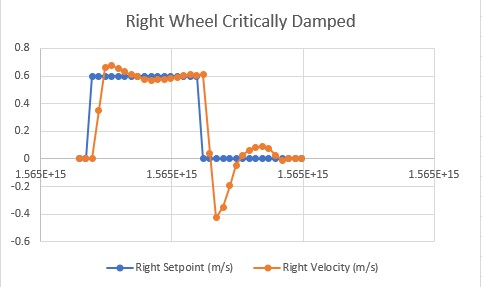
\includegraphics[width=\linewidth]{rc.jpg}
	\caption{A plot of the setpoint and velocity of the right motor exhibiting critically damped behavior}
	\label{fig:rc}
\end{figure}

\subsection{Open-Loop Control}
In open-loop control, we predetermine the motor commands to send to MBot prior to running the program. MBot only relies on such pre-programmed commands and encoder readings to execute those comamnds. No external sensory feedback like odometry or laser scans are evaluated in open-loop control.

In our program, we first decided on using $v_0 = 0.25 m/s$ as the initial desired individual wheel velocity set-point. The task of driving in a square three times can be abstracted into two tasks: driving straight and turning. When driving straight, we set both the left and right setpoints equal to the initial velocity like equation \ref{eq:sps}.
\begin{equation} \label{eq:sps}
v_{L_{sp}} = v_{R_{sp}} = v_0
\end{equation}
Since we know the distance $\Delta s = 1 m$ MBot needs to travel straight, and we determined the initial velocity $v_0 = 0.25 m/s$. The time $\Delta t_{forward}$ it takes for MBot to reach the desired travel distance is $\Delta t_{forward} = \frac{\Delta s}{v_0}$. After sending the motor commands to the left and right wheels, the program lets the motors keep those setpoints for $\Delta t_{forward}$ seconds before stopping the motors and transition to the turning task.

When turning counterclockwise, each wheel still uses the initial velocity $v_0 = 0.25 m/s$, but spins in different direction. Specifically, the left wheel spins backwards while the right wheel still spins forward. It is characterized by equation \ref{eq:spt}
\begin{equation} \label{eq:spt}
v_{L_{sp}} = -v_{R_{sp}}
\end{equation}
The time $\Delta t_{turn}$ needed for MBot to turn counterclockwise 90 degrees can be computed following equation \ref{eq:tt}
\begin{equation} \label{eq:tt}
\Delta t_{turn} = \frac{B}{v_0} * \frac{\pi}{4}
\end{equation}
In the same way as driving forward, after sending the motor commands for turning, our program lets MBot keep turning for $\Delta t_{turn}$ seconds.

To complete the square three times, four segments of driving straight forward and turning counterclockwise are needed for each square. Therefore, the two tasks are repeated 12 times. Figure \ref{fig:task4} is the screenshot of the Vx visualization of the Ded Reckoning odometry trajectory of MBot after drovomg around the square three times. 

As shown in figure \ref{fig:task4}, a well-tuned robot can approximately drive around in  a square a few times. However, the trajectory deviates over time, and the position of each turn is slightly different each time. The control law cumulates a noticeable amount of random error over time and drift in odometry over time. In the physical world, upon completion of the third square, MBot is so off course that both its wheels are outside of the square on the ground. We can conclude that the open-loop control does not perform well over time due to the cumulative internal sensor error.

\begin{figure}
	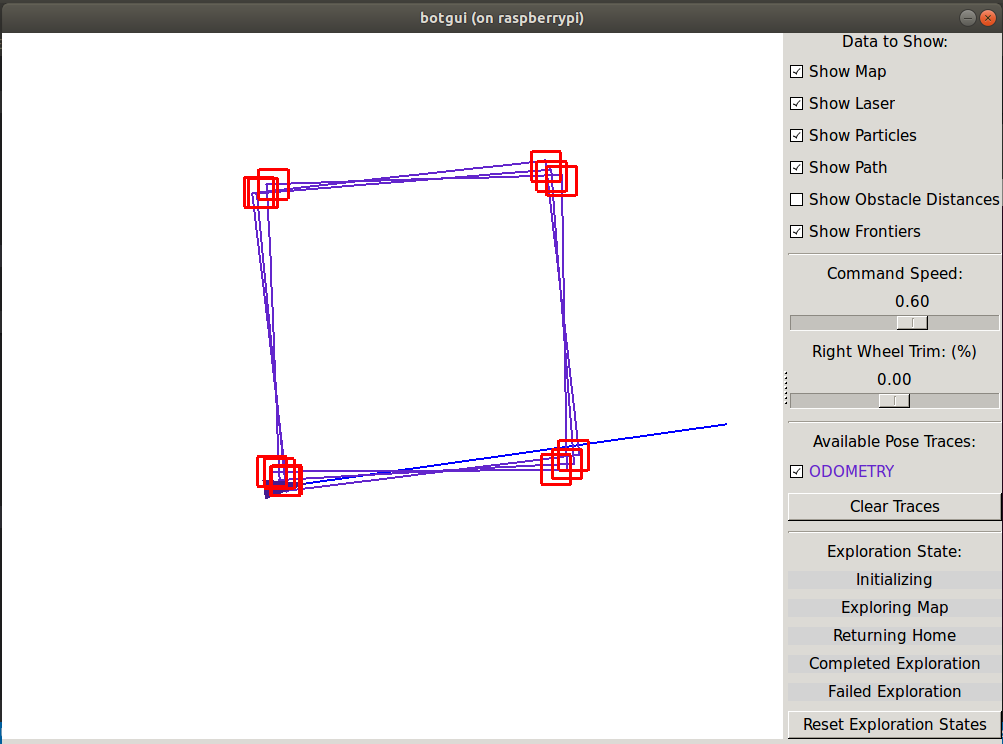
\includegraphics[width=\linewidth]{task4.png}
	\caption{A screenshot of the Vx visualization software of the perceived odometry trace of MBot after driving around a square three times under a open-loop velocity control}
	\label{fig:task4}
\end{figure}


\subsection{Closed Loop Control with Odometry}
We have seen from open-loop control that relying solely on pre-programmed commands is susceptible to cumulative error. We then implemented the closed-loop control with odometry for completing the same task of driving around a one meter square three times. The odometry feedback along with the velocity feedback give MBot some information about how it is interacting with the environment. The control law then incorporates those feedback while calculating the next motor commands to send to each motor.

Instead of generalizing the tasks into only driving straight forward and turning counterclockwise, we are now abstracting the task into different states. Our program is a finite state machine that takes MBot from one state to the next. When MBot first starts, its initial pose $(x, y, \theta)$ is set to the robot origin pose (0, 0, 0). Henceforth, the sequence of the vertices to visit can be determined for each leg of travel. The finite state machine can be further abstracted into executing commands in one state and switching between the states. There are four straight-driving states for driving and turning state in between each of them, while making a lap around the one meter square. Therefore, we use a state counter to indicate MBot's current state.

State 0 is the travel segment from (0, 0) to (1, 0) and turning counterclockwise 90 degrees. In this state, we define the error term to be the y coordinate from odometry, because hypothetically when driving straight forward, only x should increment. When driving forward, the theta term should be 0 because the current heading is 0. To determine when we should turn, we periodically check the x coordinates from the odometry reading. When the x coordinates is within epsilon $\epsilon = 0.02$ meters away from one meter, we command the MBot to turn.

State 1 is the travel segment from (1, 0) to (1, 1) and the subsequent turning. MBot should have the pose $(1, 0, \frac{\pi}{2})$ at the beginning of the state, and terminates with the pose $(1, 1, \pi)$ before entering the next state. In state 1, we define the translational error term $e$ to be the x coordinates from odometry subtracted by one meter. The rotational $\theta$ is defined as the difference between a target heading angle of $\frac{\pi}{2}$ radians and the actual heading from odometry.

State 2 is the travel segement from (1, 1) to (0, 1) and the 90-degree turn. MBot starts with the pose $(1, 1, \pi)$ and enters the next state upon reaching the pose $(0, 1, \frac{3\pi}{2})$. The translational error term $e$ is the y coordinates from odometry minus one meter. The rotational $\theta$ is the difference between the target heading of $\pi$ and the actual heading from odometry reading.

State 3, the final state before reentering state zero, is the segment from (0, 1) back to (0, 0) and the turn. MBot begins with the pose $(0, 1, \frac{3\pi}{2})$, and should terminate this state at the pose (0, 0, 0), which is the starting pose of state 0. The translational error term $e$ is defined to be the x coordinate from odometry. The rotational term $\theta$ is the difference between the target heading of $\frac{3\pi}{2}$ and the actual heading from odometry.

The states can thus run as a loop for an arbitrary number of times to drive around the square. We have introduced the unicycle model and solved for the damped spring differential equation in equation \ref{eq:um}. In this controller, to keep MBot driving on the desired path, we are setting the desired setpoints with equation \ref{eq:ddf} for the translational velocity $v$ and equation \ref{eq:ddt} where $k_1$ is the integral term and $k_2$ is the proportional gain discussed in section II. C. of this report.
\begin{equation} \label{eq:ddf}
v = v_0
\end{equation}
\begin{equation} \label{eq:ddt}
\omega = -k_1\theta-\frac{k_2}{v_0}e
\end{equation}

Different from the previous open-loop controller, instead of commanding the left and right wheels as separate setpoins, we are abstracting away the concept of wheels entirely with this closed-loop controller. For each state described above, when driving straight, we set the desired forward velocity $v = v_0 = 0.2 m/s$, and the desired angular velocity $\omega$ to be that in equation \ref{eq:ddt}. The exact motor commands are calculated by the PID controller following equation \ref{eq:dvr} for the right wheel and equation \ref{eq:dvl} for the left wheel as demonstrated in section II. B. of this report.

To turn, our program sets the desired translational velocity $v = 0$, and the desired angular velocity $\omega = \frac{\pi}{5} r/s$. It periodically checks odometry reading until MBot's current heading is within $\epsilon$ from the desired angle, after which it enters the next state.

Figure \ref{fig:task5} is the screenshot of the Vx visualization of the odometry traces after driving more than three times around the one meter square. The Ded Reckoning trajectory while driving straight the red squares indicating the turns are both more precise than those in the open-loop control. Because the closed-loop controller corrects for error based on odometry feedback, MBot is able to reach the same poses even after completing the squares a few times. The trajectories perceived by MBot almost entirely overlap one another, which is a significant improvement from the open-loop control with regards to consistancy in robot performance. The system, however, is still not perfect. Although the perceived odometry indicates the robot is driving in a near perfect square, in real-life, MBot still deviated from its original course after driving around the square more than three times. Another anomoly that is noticeable is the red squares at the bottom right corner. The single red square slightly higher than the rest was drawn when MBot first turns, and that was at the exact coordinates (1, 0). However, after completing one square, MBot has been turning consistantly a bit lower than that cooridinate. We suspect the epsilon term in our algorithm is introducing this systematic error to MBot. Nevertheless, the closed-loop control with odometry performed significantly better and more consistantly than the open-loop control.

\begin{figure}
	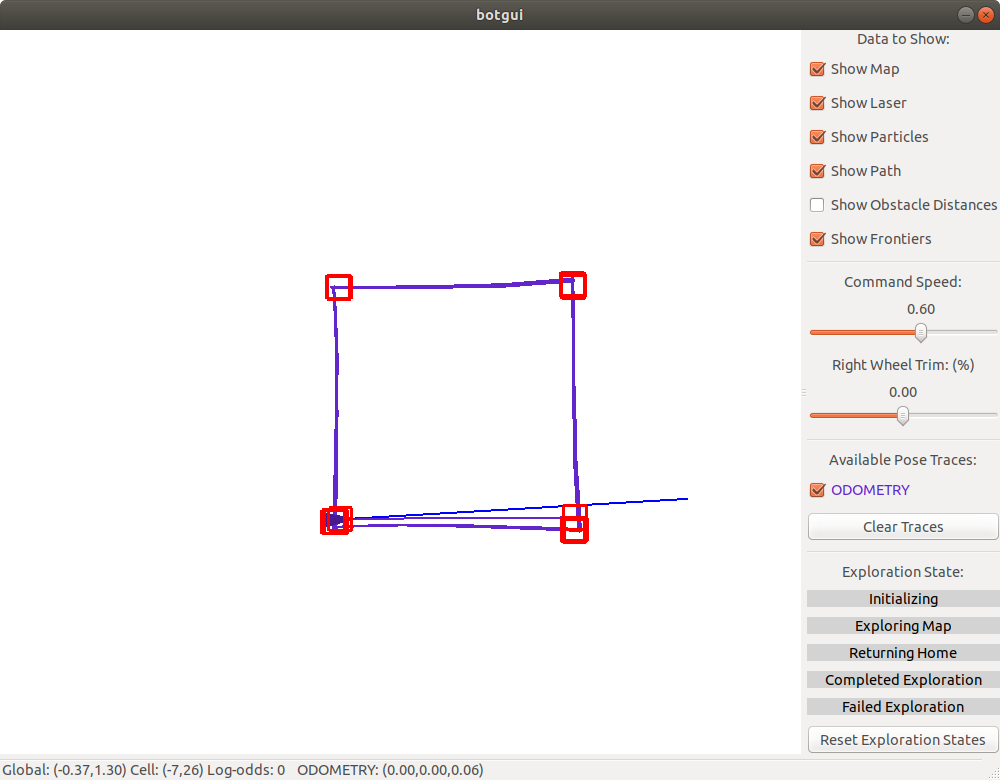
\includegraphics[width=\linewidth]{task5.png}
	\caption{A screenshot of the Vx visualization software of the perceived odometry trace of MBot after driving around a square more than three times under closed-loop control with odometry}
	\label{fig:task5}
\end{figure}


\subsection{Closed Loop Control with Laser Scans}
We implemented the closed-loop control using laser scans based on the closed-llop control with odometry. The new controller requires us to overcome two technical challenges, namely driving straight with the wall follower algorithm, and turning.

For driving straight, we modified the same wall follower control algorithm described in the closed-loop odometry section. We defined a new method for calculating $\theta$ and $e$ using only the lidar. In our program, the lidar scans two separate $20^{o}$ circular arcs, one in the positive $y$ direction relative to the robot (to its right) and the other in the positive $x$ direction (directly towards its front). Within these $20^{o}$ arcs, our program then iterates through each distance value and search for the minimum distance and the corresponding angle relative to the coordinate system of the robot. We are using $20^{o}$ arcs because the wider range allows for up to $10^{o}$ of deviation from a straight path while still allowing the robot to find the true local minimum distances. We are not using a larger angle since if MBot deviates from the straight path near a corner, the wall to its front may be inside the view of the side sector, which could cause the robot to find an incorrect local minimum distance and angle. The wall follower algorithm uses the front arc and the  corresponding local minimum distance to determine when to stop going forward and transition into the turning state. More specifically, the robot advances forward until the minimum distance inside the front cone is equal to the minimum on the side.

The challenge of knowing when MBot should stop turning is solved with a constraint based approach. First, we save the distance from the front of the robot to the wall immediately prior to turning (once the robot is stationary after wall following). The point-turn is initialized and the robot is assumed to maintain a translational velocity of 0. The first constraint that must be satisfied to stop the point-turn is that the distance to the side wall is equal to the saved distance to the front wall to within some margin. The second constraint is that the distance to a wall to the right of the robot should be at least $20\%$ greater than the distance from the side wall before the robot starts turning. The value of $20\%$ is chosen because when the walls converge to a corner, the maximum distance should be $~\sqrt{2} \times \approx 1.4$ times the distance to the side wall and $\frac{1.4 - 1}{2} = 20\%$.


To determine the state transition, we maintain two local minima, a front minimum distance and a side minimum distance. The minima are calculated by the lidar scanner readings in the range between $[-\delta, \delta]$ and $[\frac{\pi}{2} -\delta,\frac{\pi}{2} + \delta] $ respectively. $\delta$ is a deviation parameter, which is 10 degrees in this implementation. The algorithm is as follows:

\begin{algorithm}[H]
	\caption{Handle lidar}
	\begin{algorithmic}
		\STATE $S, D_{side}, D_{front}, about \; turning = False$
		
		\IF{$S = DRIVING$}
		\IF{$D_{front} - D_{side} < 0$}
		
		\STATE $S = TURN$, $Is \; Turning = False$
		\ENDIF
		\ELSIF{$S = TURN$}
				\IF{$D_{side} > \gamma$ }
		\STATE $Is \; Turning = True$
		\ENDIF
		\IF{$|D_{side} - D_{before \; turn}| < \delta$ and $Is \; Turning$}
		\STATE $S = DRIVING$
		\ENDIF
		\ELSE
		\STATE $S = STOP$
		\ENDIF
	\end{algorithmic}
\end{algorithm}

For turning, we set the motor commands to constant. For the driving controller, we maintain the method we use for odometry (PD controller based on $\theta$ and error). We have 
$$
error = dD_{side}
$$
$$
error_{\theta} = \frac{\pi}{2} - \theta_{side}
$$
where $dD_{side}$ is difference of local minimum distance on the side between each state, and $\theta_{side}$ is the angle of the minimum from the driving direction.

For drawing the trajectory, we mark the starting point to be the origin of the frame of reference, and then we assign x and y to the corrsponding front and side distance we get from the lidar.
For theta, since we didn't figure out a reliable way to caculate it accurately, we simply assign it to one of $\frac{\pi}{2},\pi,\frac{3\pi}{2},2\pi$

\begin{figure}
	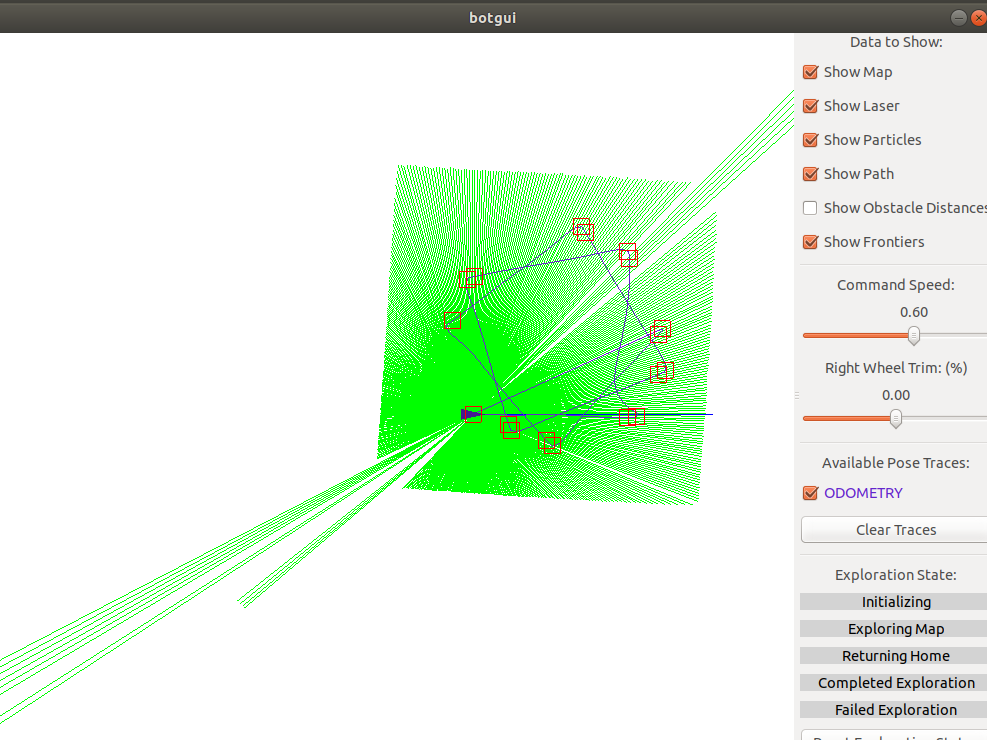
\includegraphics[width=\linewidth]{task6_1.png}
	\caption{A screenshot of the Vx visualization software of the poses perceived by only odometry.}
	\label{fig:task6_1}
\end{figure}

\begin{figure}
	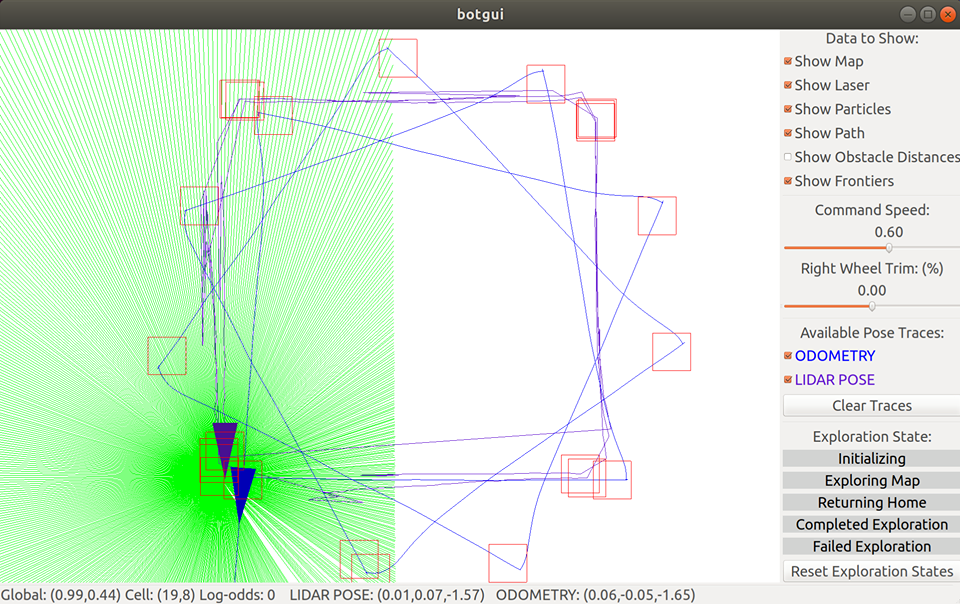
\includegraphics[width=\linewidth]{task6_2.png}
	\caption{A screenshot of the Vx visualization software of the poses perceived by odometry and the Lidar.}
	\label{fig:task6_2}
\end{figure}

As you can see in figure \ref{fig:task6_2}, the odometry traces appear drastically different from the laser scan trajectory. In the closed-loop control with odometry,
the controller adjusts the robot trajectory such that the internally perceived Ded Reckoning trajectory matches the desired path. As a result, figure \ref{fig:task5}
for the closed-loop odometry control looks like perfect squares. For the visualization of the closed-loop contnrol with lidar, the robot trajectory is adjusted based on
actual the lidar readings of the external world without any consideration for odometry. As a result, the odometry traces in figure \ref{fig:task6_2} is almost completely
different from that of the laser scan trajectory.


\section{Discussion}
We have so far implemented the closed-loop velocity control law, open-loop control, closed-loop control with odometry, and closed-loop control with laser scans.
With closed-loop velocity control, we have tuned the PID such that the each motor exhibits dcritically damped behavior. We have shown that although it is feasible
to drive MBot using an open-loop controller, the robot is susceptible to random dynamic factors in the environemnt or the motor. The closed-loop control with odometry
performces better as it corrects for the errors based on the feedback from the internal encoder readings. However, the deduced odometry drifts from the real world 
coordinates due to factors such as the wheels slipping, and cannot be detected with internal sensors. These error cumulates and can cause the robot to go off course 
over time. On the other hand, closed-lop control with only laser scans relies only on the external sensory feedback from the laser range finder. We implemented the
wall-follower algorithm under the unicycle for the controller. We have found that while the wall-follower is a good controller for driving straight, estimating current
heading based on lidar readings is less reliable than that from odometry. Therefore, we used a combination of odometry deduced from internal encoder readings and the 
robot pose estimated based on an external lidar range sensor for our challenge. Driving straight with the wall-follower with lidar and turning with odometry yielded the 
optimal results. Furthermore, we have exhibited from our visualization software and real-world observasions that there is a difference between MBot's perceived Ded Reckoning
trajectory based on odometry and estimated trajectory based on external lidar readings, and that of the actual pose of MBot in the physical world. Therefore, we cannot rely
on one model or sensor for selecting control laws, but should rather implement a combination of the sensory data available to the mobible robot.


\appendix
\section{Certification}
\begin{figure}
	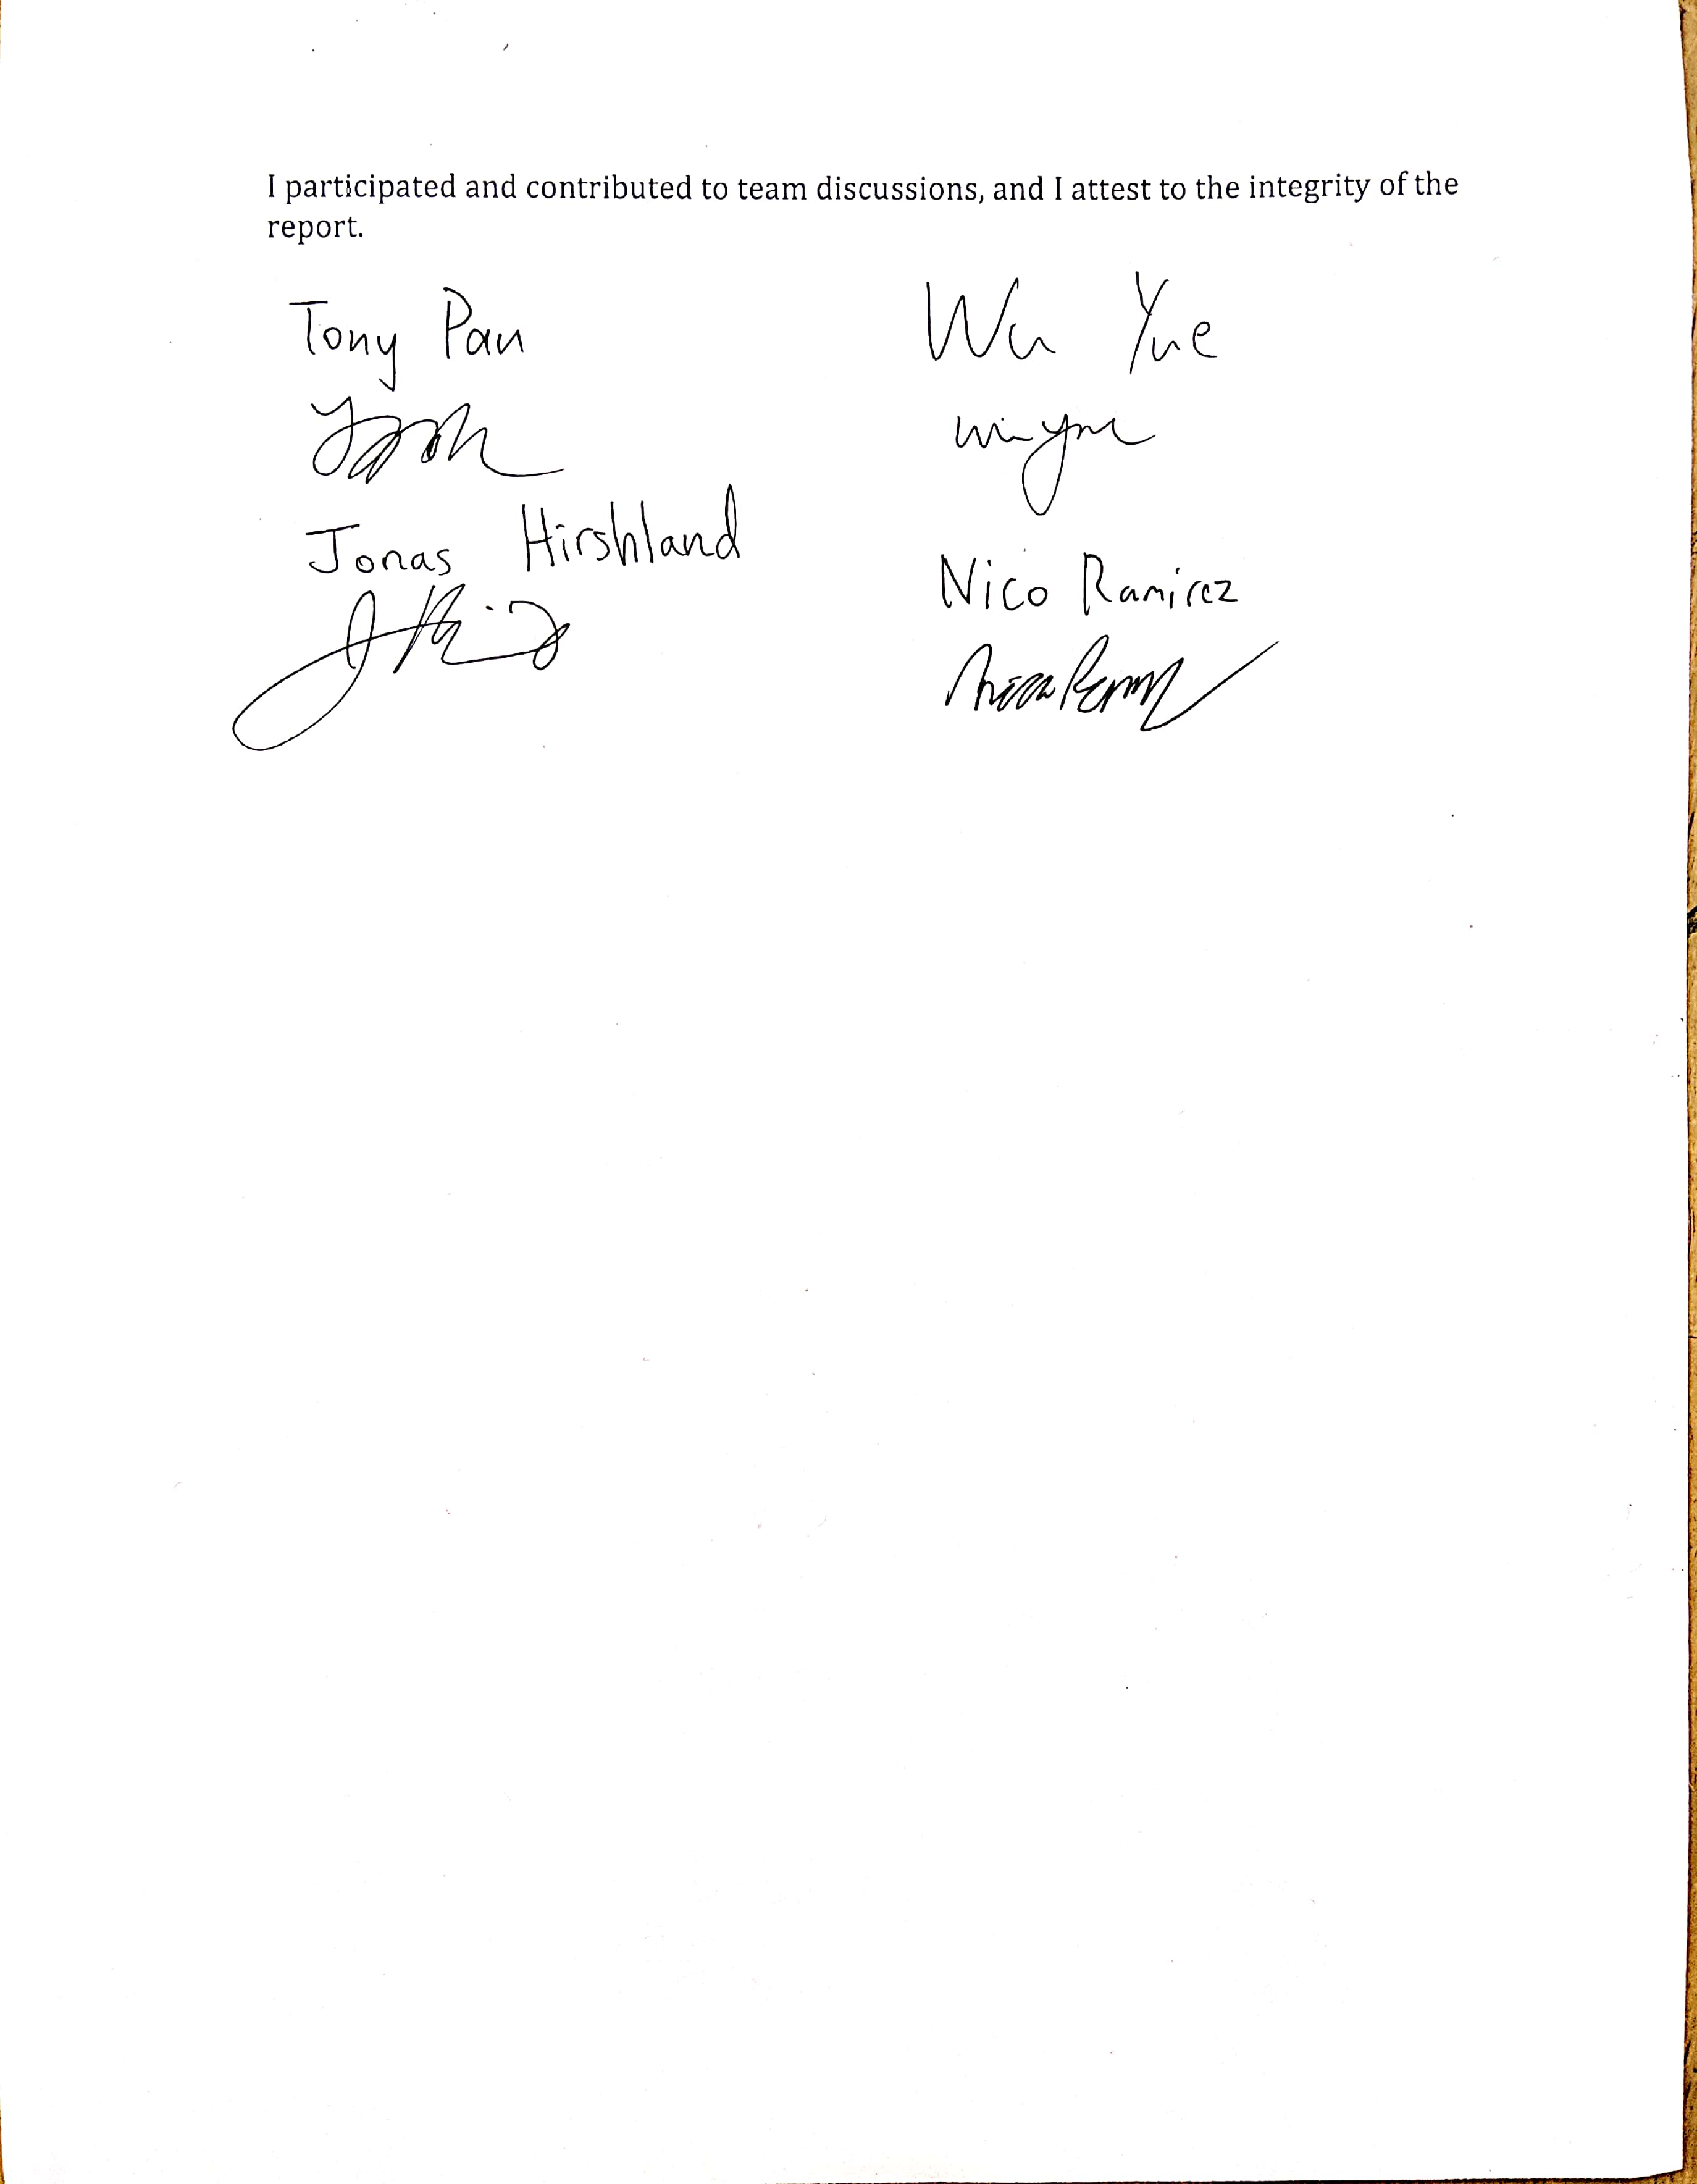
\includegraphics[width=\linewidth]{certification.jpg}
\end{figure}

\bibliographystyle{IEEEtran}
\bibliography{references.bib}



\clearpage
%%%%%%%%%%%%%%%%%%%%%%%%%%%%%%%%%%%%%%APPENDIX%%%%%%%%%%%%
\begin{appendices}
\onecolumn
\end{appendices}

\end{document}
